\documentclass{ximera}
\usepackage{sagetex}
%% handout
%% space
%% newpage
%% numbers
%% nooutcomes
 
%% You can put user macros here
%% However, you cannot make new environments

\graphicspath{{./}{module1Activity/}{module2Activity/}{module3Activity/}}

\usepackage{sagetex}
\usepackage{tikz}
\usepackage{hyperref}
\usepackage{tkz-euclide}
\usetkzobj{all}
\pgfplotsset{compat=1.7} % prevents compile error.

\tikzstyle geometryDiagrams=[ultra thick,color=blue!50!black]
 %% we can turn off input when making a master document
 
\outcome{}
\author{Darryl Chamberlain Jr.}
  
\title{Objective 1 - Identify Type of Model}
 
\begin{document}
\begin{abstract}

\end{abstract}

\maketitle
 
\textit{Note: There are no textbook or videos directly to this section. If you want to review a certain type of model, you will need to go back to that Module.}
 
%%%%%%%%%%%%%%%%%%%%%
%%%  Objective 1  %%%
%%%%%%%%%%%%%%%%%%%%%

We summarize the types of models we've looked at below. 

\textbf{Linear Model:}
\begin{itemize}
    \item Used when we have a \textit{constant} variation between two quantities. 
    \item $y = mx + b$. Can be multiple lines added together. 
    \item Phrases to look for: consant, steadily increasing/decreasing, adding/subtracting [/, /,] every [/, /,].
\end{itemize}

\textbf{Direct Variation:}
\begin{itemize}
    \item Used when we have a \textit{direct} variation between two quantities (as one quantity increases, the other increases).
    \item $y = kx^n$. Joint variation may have more than one variable (like $y = kx^n z^m$)
    \item Phrases to look for: vary directly, directly proportional, ``as one increases, so does the other".
\end{itemize}

\textbf{Inverse Variation:}
\begin{itemize}
    \item Used when we have an \textit{indirect} variation between two quantities (as one quantity increases, the other decreases). 
    \item $y = \frac{k}{x^n}$. Combined with joint variation, there may be more than one variable (like $PV=nRT$). 
    \item Phrases to look for: vary indirectly, directly proportional, ``as one increases, the other decreases". 
\end{itemize}

\textbf{Logarithmic Model:}
\begin{itemize}
    \item Used when we have a \textbf{rapid} early growth, then slower growth later. 
    \item $y = \log(kx)$. Remember that $\ln(x) = \log_e(x)$. 
    \item Phrases to look for: rapid early growth/decay, no bound on growth/decay.
\end{itemize}

\textbf{Exponential Model:}
\begin{itemize}
    \item Used when we have a slow initial growth, then \textit{rapid} growth later.
    \item $y = a^{kx}$. Common bases are 2, 3, and $e$.
    \item Phrases to look for: rapid late growth/decay, bounds on growth/decay.
\end{itemize}

%\textbf{General Function Model:}
%\begin{itemize}
%    \item Used when the problem specifies to use a particular function to estimate the data. 
%    \item Use the general form of the function. For example, if using quadratic function to model data, use $y = ax^2+bx+c$. 
%    \item You may need to solve a system of equations to construct the model. A short review of Substitution and Elimination will be included in the next Objective. 
%\end{itemize}

Determine the type of model that would be most appropriate for each situation below. Answers will be either:
\begin{itemize}
    \item Linear 
    \item Direct
    \item Indirect
    \item Logarithmic
    \item Exponential
    \item General (if we are going to use the general form of a particular function)
\end{itemize}

\begin{question}
Your bank offers a savings account that will increase your total balance by 0.2\% annually. You want to decide how much to initially deposit and if the initial deposit makes a big difference in the long run. S

$\answer[format=string]{Exponential}$

\end{question}

\begin{question}
A ball is dropped from the top of Century Tower. The ball steadily picks up speed before hitting the ground. You want to figure out what the ball's height is at a certain time.

$\answer[format=string]{Direct}$

\end{question}


\begin{question}
Chemists commonly create a solution by mixing two products of differing concentrations together. For example, a chemist could have large amounts of a 10\% acid solution and a 30\% acid solution, but need a 10 liter 15\% solution. 

$\answer[format=string]{Linear}$

\end{question}

\begin{question}
[Astronomy] Kepler's Third Law: The square of the time, $T$, required for a planet to orbit the Sun is directly proportional to the cube of the mean distance, $a$, that the planet is from the Sun. 

$\answer[format=string]{Direct}$

\end{question}

\begin{question}
[Physics] The rate of vibration of a string under constant tension, $r$, varies inversely with the length of the string, $l$.

$\answer[format=string]{Indirect}$

\end{question}


\begin{question}
A population of bacteria doubles every hour. 

$\answer[format=string]{Exponential}$

\end{question}

\begin{question}
[Anthropology] Radiocarbon dating is used to calculate the approximate date a plant or animal died by noting the percentage of carbon-14, $r$ in the object. The age of the object $t$, in years, is directly proportional to the natural log of the percentage of carbon-14, $r$ in the object. 

$\answer[format=string]{Logarithmic}$

\end{question}

\begin{question}
The weight of an object above the surface of Earth varies inversely with the square of the distance from the center of Earth. 

$\answer[format=string]{Indirect}$

\end{question}

\begin{question}
The kinetic energy $K$ of a moving object varies jointly with its mass $m$ and the square of its velocity $v$.

$\answer[format=string]{Direct}$

\end{question}

\begin{question}
Carlos has taken an initial dose of a prescription medication orally. The medicine is absorbed rapidly by the large intestine and absorbed slowly as it is digested otherwise. 

$\answer[format=string]{Exponential}$

\end{question}

\begin{question}
\begin{figure}
	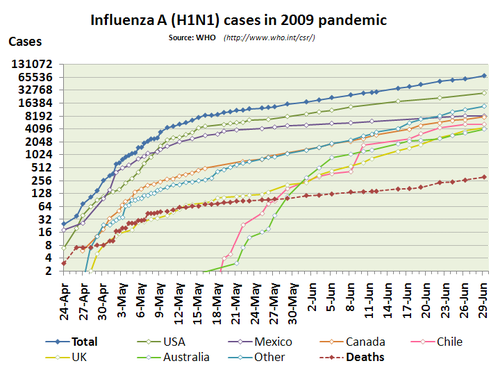
\includegraphics[scale=0.75]{Influenza-2009.png}
\end{figure}

$\answer[format=string]{Logarithmic}$

\end{question}

\begin{question}
A ball is dropped from the top of Century Tower. The ball steadily picks up speed before hitting the ground. You want to figure out what the ball's speed is at a certain time.

$\answer[format=string]{Linear}$
\end{question}

\begin{question}

\begin{figure}
	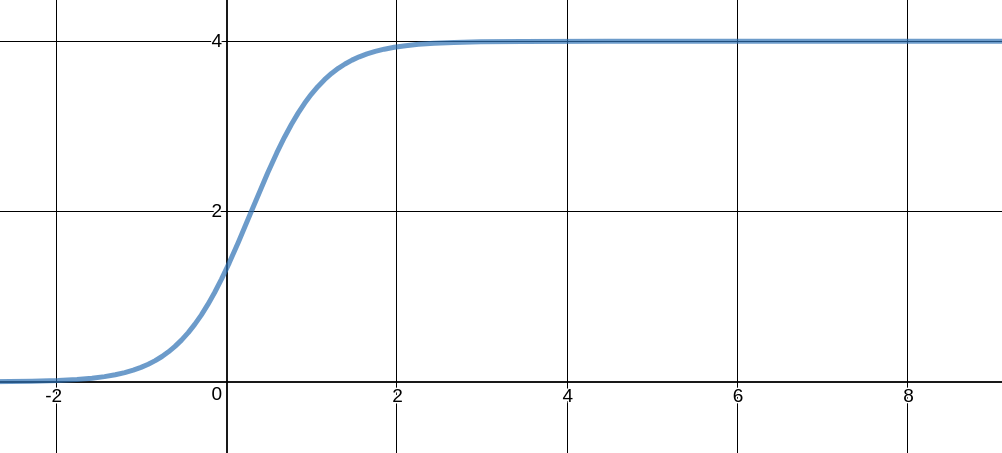
\includegraphics[scale=0.5]{logarithmicGrowth.png}
	\caption{A sigmodial curve.}
\end{figure}

$\answer[format=string]{Exponential}$

\end{question}

\begin{question}
Kappa Delta is hosting an all-you-can-eat pancake fundraiser to support the prevention of child abuse. Adult (18+) tickets are \$10 and teen (10-17) tickets are \$5. Children under 10 are let in without a ticket. The ticket-sellers only keep track of the total number of tickets sold and total revenue, but want to know how many adult and teen tickets were sold. 

$\answer[format=string]{Linear}$

\end{question}

\end{document}